\documentclass[presentation,10pt]{beamer}
%\documentclass[hyperref=unicode, handout,10pt]{beamer}
%\usepackage{handoutWithNotes}

\mode<presentation>{\usetheme{default}
 \usecolortheme{whale}}

%BEGIN HANDOUT
\mode<handout>
{
\usetheme{default}
 \usecolortheme{default}

  \usepackage{pgf}
  \usepackage{pgfpages}

\pgfpagesdeclarelayout{4 on 1 boxed}
{
  \edef\pgfpageoptionheight{\the\paperheight} 
  \edef\pgfpageoptionwidth{\the\paperwidth}
  \edef\pgfpageoptionborder{0pt}
}
{
  \pgfpagesphysicalpageoptions
  {%
    logical pages=4,%
    physical height=\pgfpageoptionheight,%
    physical width=\pgfpageoptionwidth%
  }
  \pgfpageslogicalpageoptions{1}
  {%
    border code=\pgfsetlinewidth{2pt}\pgfstroke,%
    border shrink=\pgfpageoptionborder,%
    resized width=.5\pgfphysicalwidth,%
    resized height=.5\pgfphysicalheight,%
    center=\pgfpoint{.25\pgfphysicalwidth}{.75\pgfphysicalheight}%
  }%
  \pgfpageslogicalpageoptions{2}
  {%
    border code=\pgfsetlinewidth{2pt}\pgfstroke,%
    border shrink=\pgfpageoptionborder,%
    resized width=.5\pgfphysicalwidth,%
    resized height=.5\pgfphysicalheight,%
    center=\pgfpoint{.75\pgfphysicalwidth}{.75\pgfphysicalheight}%
  }%
  \pgfpageslogicalpageoptions{3}
  {%
    border code=\pgfsetlinewidth{2pt}\pgfstroke,%
    border shrink=\pgfpageoptionborder,%
    resized width=.5\pgfphysicalwidth,%
    resized height=.5\pgfphysicalheight,%
    center=\pgfpoint{.25\pgfphysicalwidth}{.25\pgfphysicalheight}%
  }%
  \pgfpageslogicalpageoptions{4}
  {%
    border code=\pgfsetlinewidth{2pt}\pgfstroke,%
    border shrink=\pgfpageoptionborder,%
    resized width=.5\pgfphysicalwidth,%
    resized height=.5\pgfphysicalheight,%
    center=\pgfpoint{.75\pgfphysicalwidth}{.25\pgfphysicalheight}%
  }%
}


  \pgfpagesuselayout{4 on 1 boxed}[a4paper, border shrink=5mm, landscape]
  \nofiles
}
%END HANDOUT


\usepackage[absolute,overlay]{textpos}
\usepackage{array}
\usepackage{graphicx}
\usepackage{adjustbox}
\usepackage[version=3]{mhchem}
\usepackage{chemfig}
\usepackage{textcomp}
\usepackage{ucs}
\usepackage[utf8]{inputenc}
\usepackage{multirow}

\PrerenderUnicode{ěščřžýáíéĚŠČŘŽÝÁÍÉďťňĎŤŇůúÚóÓ}

\usepackage{fontspec} 
\usepackage{unicode-math}

\usepackage{polyglossia}
\setdefaultlanguage{czech}

\def\uv#1{„#1“}

\setbeamertemplate{footline}[frame number]

\addtobeamertemplate{frametitle}{
   \let\insertframetitle\insertsectionhead}{}
\addtobeamertemplate{frametitle}{
   \let\insertframesubtitle\insertsubsectionhead}{}

\makeatletter
  \CheckCommand*\beamer@checkframetitle{\@ifnextchar\bgroup\beamer@inlineframetitle{}}
  \renewcommand*\beamer@checkframetitle{\global\let\beamer@frametitle\relax\@ifnextchar\bgroup\beamer@inlineframetitle{}}
\makeatother
\setbeamercolor{section in toc}{fg=blue}
\setbeamertemplate{section in toc shaded}[default][100]

\begin{document}
\title[Crisis] % (optional, only for long titles)
{Vyhodnocování IR a RA spekter}

\author % (optional, for multiple authors)
{Zdeněk Moravec, Ústav chemie, PřF MU \\ hugo@chemi.muni.cz \\
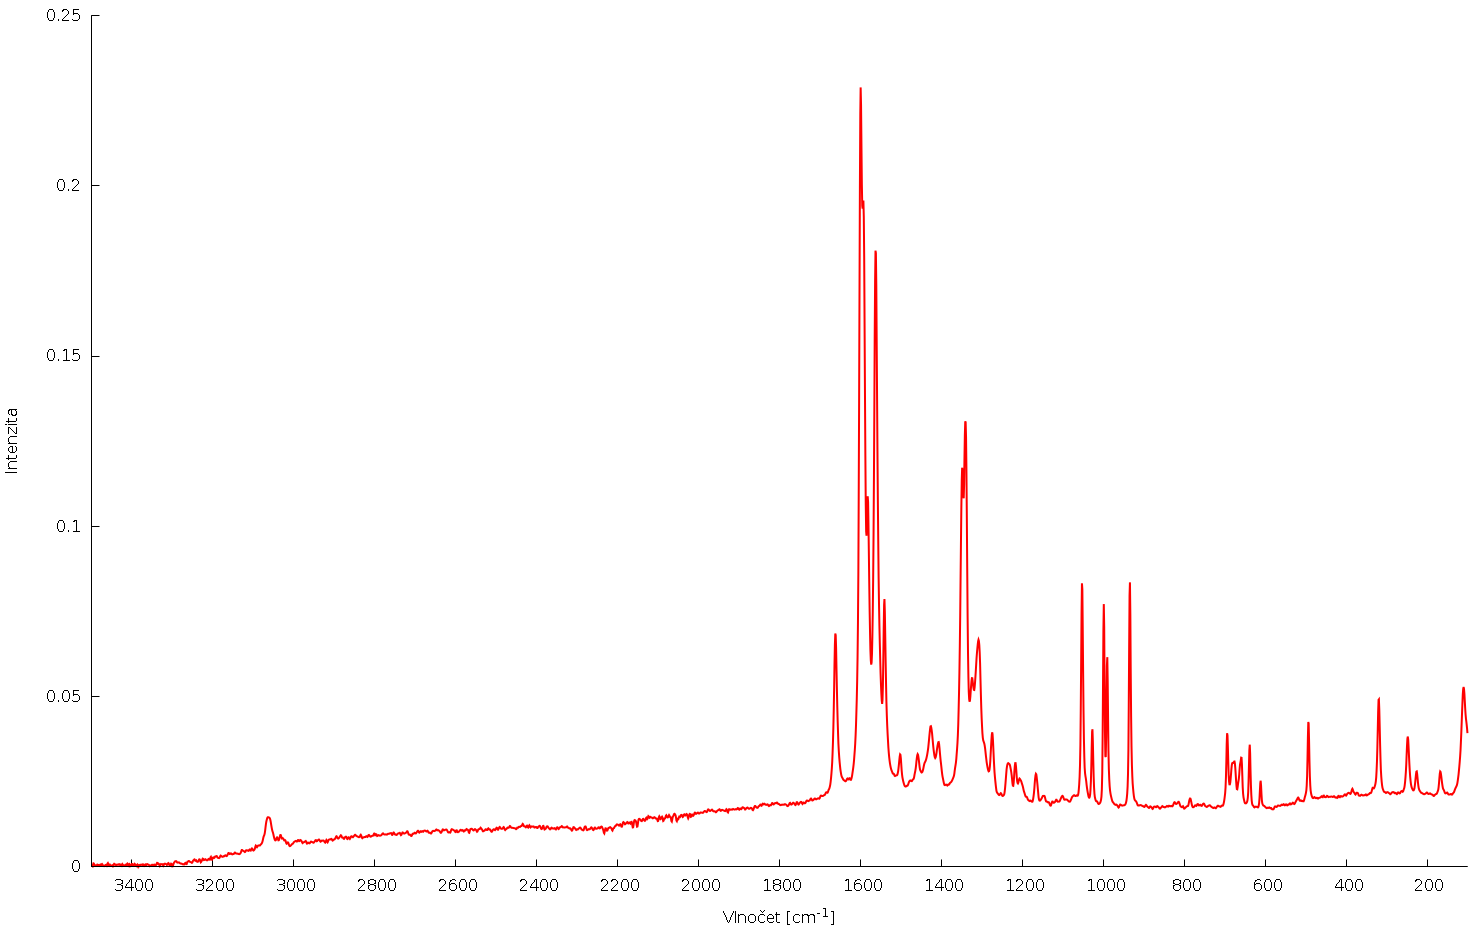
\includegraphics[width=85mm]{img/raman-spect.png}}
%{http://z-moravec.net}

\date{ } %hide date on titlepage

%\subtitle{Metody chemické výzkumu}

\frame{\titlepage}

\section{Úvod}
\frame{
	\frametitle{}
	\vfill
	\begin{itemize}
		\item Vzorky, u kterých neznáme ani přibližné složení, lze pomocí IR a RA spektroskopie analyzovat s využitím databází spekter.
		\item Pokud máme alespoň přibližnou představu o struktuře vzorku, lze spektra využít pro potvrzení nebo vyvrácení přítomnosti funkčních skupin a pro kontrolu čistoty reaktantů a produktů.
	\end{itemize}
	\begin{center}
	\adjincludegraphics[width=115mm]{img/irBandsOrg.png}
	\end{center}
	\vfill
}

\section{Kvalitativní analýza}
\subsection{Rozdělení oblastí spekter}
\frame{
	\frametitle{}
	\vfill
	\begin{itemize}
	\item  NIR (0,7 -- 2,5 $\mu$m; 14 000 - 4 000 cm$^{-1}$) - infračervená spektroskopie v blízké oblasti -- převážně overtony a kombinační vibrace. Intenzita pásů je nižší než v MIR oblasti a pásy se často překrývají.
	\item  \textbf{MIR (2,5 -- 25 $\mu$m; 4 000 - 400 cm$^{-1}$) - infračervená spektroskopie ve střední oblasti} -- základní vibrace molekul.
	\item  FIR (25 -- 1000 $\mu$m; 400 - 10 cm$^{-1}$) - infračervená spektroskopie ve vzdálené oblasti -- vibrace vazeb kov-halogen, deformační vibrace skeletu molekul.
	\end{itemize}
	\vfill
}

\subsection{Databáze spekter}
\frame{
	\frametitle{}
	\vfill
	\begin{itemize}
		\item Pokud známe předpokládané složení vzorku, je možné využít databáze spekter a provést srovnání spektra naše vzorku s tabelovaným spektrem.
		\item Je vhodné, aby byla obě spektra naměřená stejnou technikou.
		\item Databáze jsou často placené nástroje, které umožňují vyhledávání a srovnávání spekter.
		\item Databáze dostupné bez poplatku umožňují zpravidla pouze prohlížení spekter.
	\end{itemize}
	\vfill
}

\frame{
	\frametitle{}
	\vfill
	\begin{itemize}
		\item \href{http://sdbs.riodb.aist.go.jp/sdbs/cgi-bin/cre\_index.cgi}{sdbs.riodb.aist.go.jp/sdbs/cgi-bin/cre\_index.cgi}
	\end{itemize}
	\adjincludegraphics[width=10cm,valign=l]{img/sdbs.png}
	\vfill
}

\frame{
	\frametitle{}
	\vfill
	\begin{itemize}
		\item \href{http://sdbs.riodb.aist.go.jp/sdbs/cgi-bin/cre\_index.cgi}{sdbs.riodb.aist.go.jp/sdbs/cgi-bin/cre\_index.cgi}
	\end{itemize}
	\adjincludegraphics[width=12cm,valign=l]{img/sdbs2.png}
	\vfill
}

\frame{
	\frametitle{}
	\vfill
	\begin{itemize}
		\item \url{http://webbook.nist.gov/chemistry/}
	\end{itemize}
	\adjincludegraphics[width=6cm,valign=l,frame]{img/nist.png}
	\vfill
}

\frame{
	\frametitle{}
	\vfill
	\begin{itemize}
		\item \url{http://webbook.nist.gov/chemistry/}
	\end{itemize}
	\adjincludegraphics[width=11.5cm,valign=l,frame]{img/nist2.png}
	\vfill
}

\subsection{Základní pravidla pro interpretaci vibračních spekter}
\frame{
	\frametitle{}
	\vfill
	\begin{enumerate}
		\item Pokud známe alespoň přibližnou strukturu vzorku, je možné provést interpretaci s využitím charakteristických frekvencí funkčních skupin.
		\item Předpokládáme, že poloha absorpčního pásu dané skupiny je minimálně ovlivněna zbytkem molekuly a nalézá se vždy ve stejné oblasti.
	\end{enumerate}
	\begin{center}
	\adjincludegraphics[width=100mm]{img/irBandsOrg.png}
	\end{center}
	\vfill
}

\frame{
	\frametitle{}
	\vfill
	\begin{enumerate}
		\item  Nejprve se podívejte na oblast vyšších vlnočtů ($>$1500 cm$^{-1}$) a hledejte výrazné pásy.
		\item  Pro každý významný pás si připravte seznam možných přiřazení.
		\item  Oblast nižších vlnočtů použijte pro potvrzení nebo vyvrácení přítomnosti funkčních skupin.
		\item \textit{Nesnažte se přiřadit každý pás ve spektru.}
		\item Pokud je to možné, hledejte pro každou funkční skupinu více pásů, např. aldehydy by měly mít pás okolo 1730~cm$^{-1}$ a zároveň i pás v oblasti 2900-2700~cm$^{-1}$. Pokud některý z pásů chybí, skupina pravděpodobně ve struktuře přítomna není.
		\item Intenzity pásů berte v úvahu pouze orientačně.
		\item \textit{V závislosti na technice měření a stavu vzorku (kapalný, pevný, roztok) může docházet k malým změnám v poloze pásů.}
		\item Pozor na pásy náležející rozpouštědlu.
	\end{enumerate}
	\vfill
}

\subsection{Interpretace vibračních spekter organických sloučenin}
\frame{
	\frametitle{}
	\vfill
	\begin{itemize}
	\item 4000-2500 cm$^{-1}$ oblast valenčních vibrací X-H
	\item 2500-2000 cm$^{-1}$ oblast trojných vazeb
	\item 2000-1500 cm$^{-1}$ oblast dvojných vazeb
	\item 1500-600 cm$^{-1}$ oblast otisku prstu (fingerprint)
	\end{itemize}
	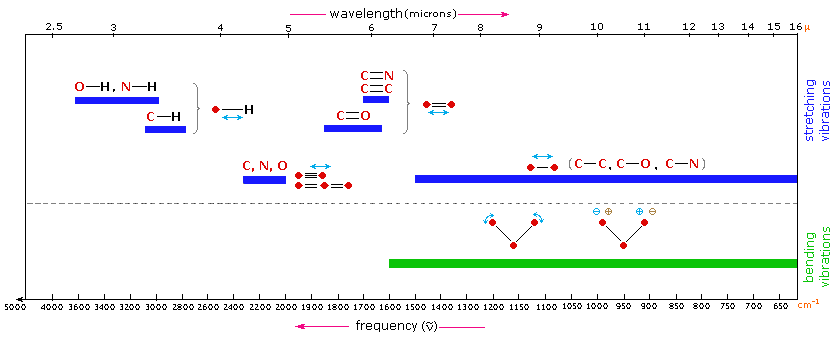
\includegraphics[width=85mm]{img/irBandsOrg.png}
	\vfill
}

\frame{
	\frametitle{}
	\vfill
	\adjincludegraphics[width=115mm,valign=l]{img/tab.png}
	\vfill
}

\frame{
	\frametitle{}
	\vfill
	\begin{tabular}{|l|l|l|}
	\hline
	\textbf{Sloučenina} & \textbf{Skupina} & \textbf{Vlnočet [cm$^{-1}$]} \\\hline
	\multirow{2}{*}{Alkany} & \ce{C-H} & 2850-3000 \\ 
	& \ce{C-C} & 800-1000 \\\hline
	\multirow{2}{*}{Aromáty} & \ce{C-H} & 3000-3100 \\ 
	& \ce{C=C} & 1450-1600 \\\hline
	\multirow{2}{*}{Alkeny} & \ce{C-H} & 3080-3140 \\ 
	& \ce{C=C} & 1630-1670 \\\hline
	\multirow{2}{*}{Alkyny} & \ce{C-H} & 3300-3320 \\ 
	& \ce{C\bond{3}C} & 2100-2140 \\\hline
	\multirow{2}{*}{Alkoholy} & \ce{O-H} & 3300-3600 \\ 
	& \ce{C-O} & 1050-1200 \\\hline
	\multirow{2}{*}{Alkyny} & \ce{C-H} & 3300-3320 \\ 
	& \ce{C\bond{3}C} & 2100-2140 \\\hline
	\multirow{2}{*}{Aldehydy} & \ce{C=O} & 1720-1740 \\ 
	& \ce{C-H} & 2700-2900 \\\hline
	\multirow{3}{*}{Karboxylové kyseliny} & \ce{C=O} & 1700-1725 \\ 
	& \ce{O-H} & 2500-3300 \\
	& \ce{C-O} & 1100-1300 \\\hline
	\end{tabular}
	\vfill
}

\frame{
	\frametitle{}
	\vfill
	\begin{enumerate}
		\item Absorpční pásy v oblasti 3200--2700~cm$^{-1}$ prokazují přítomnost alifatických (pod 3000~cm$^{-1}$) nebo aromatických (nad 3000~cm$^{-1}$) \ce{C-H} vazeb.
		\item Absorpční pásy v oblasti 3650--3250~cm$^{-1}$ prokazují přítomnost \ce{O-H} a \ce{N-H} vazeb.
		\item Absorpční pásy v oblasti 1850--1650~cm$^{-1}$ prokazují přítomnost \ce{C=O} vazeb. V této oblasti může docházet k interferenci s vazbami \ce{C=N} a \ce{N=N}, např. v purinech a azo- sloučeninách.
		\item Absorpční pásy v oblasti 1670--1620~cm$^{-1}$ prokazují přítomnost alifatických, nenasycených \ce{C=C} vazeb. Zároveň by měl být přítomen absorpční pás o vlnočtu vyšším než 3000~cm$^{-1}$.
		\item Absorpční pásy v oblasti 1615--1495~cm$^{-1}$, společně s absorpčním pásem o vlnočtu vyšším než 3000~cm$^{-1}$ prokazují přítomnost aromatických vazeb.
		\item Absorpční pásy v oblasti 2300--1990~cm$^{-1}$, ukazují na přítomnost kumulovaných násobných vazeb mezi uhlíkem nebo dusíkem, např. kyanatanů, isokyanatanů, apod.
	\end{enumerate}
	\vfill
}

\subsubsection{Aromatické sloučeniny}
\frame{
	\frametitle{}
	\vfill
	\begin{tabular}{|l|l|}
	\hline
	\textbf{Vibrace} & \textbf{Vlnočet [cm$^{-1}$]} \\\hline
	\ce{C-H} arom. valenční & 3100-3000 \\\hline
	\ce{C-H} alif. valenční & 3000-2900 \\\hline
	Kombinační, overtony & 2000-1700 \\\hline
	\ce{C=C} & 1650-1430 \\\hline
	\ce{C-H} deformační v rovině kruhu & 1275-1000 \\\hline
	\ce{C-H} deformační mimo rovinu kruhu & 900-690 \\\hline
	\end{tabular}
	\begin{columns}
	\column{.8\textwidth}
	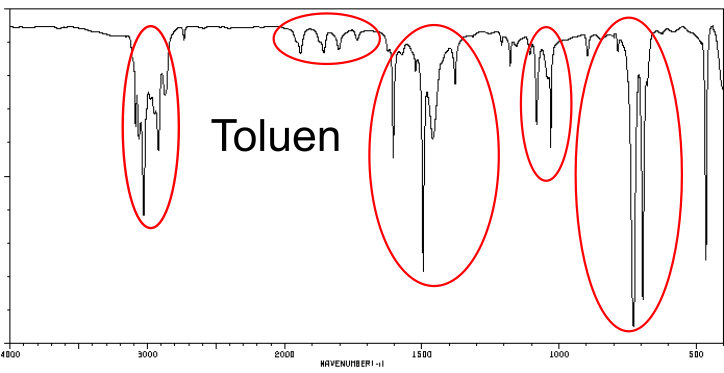
\includegraphics[width=85mm]{img/toluene.png}
	\column{.18\textwidth}
	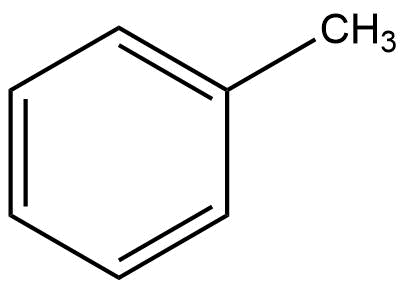
\includegraphics[width=26mm]{img/toluene-struct.png}
	\end{columns}
	\vfill
}

\subsection{Anorganické sloučeniny}
\frame{
	\frametitle{}
	\vfill
	\begin{itemize}
		\item Spektra anorganických sloučenin zpravidla obsahují méně pásů, ty jsou širší a nalézáme je i na nižších vlnočtech, často až ve FIR oblasti.
		\item Látky obsahující pouze iontovou vazbu, např. NaCl, neposkytují IR spektrum v MIR oblasti. Pozorovatelné jsou pouze mřížkové vibrace.
		\item Stupeň hydratace sloučeniny ovlivňuje vzhled spektra.
	\end{itemize}
	\begin{center}
		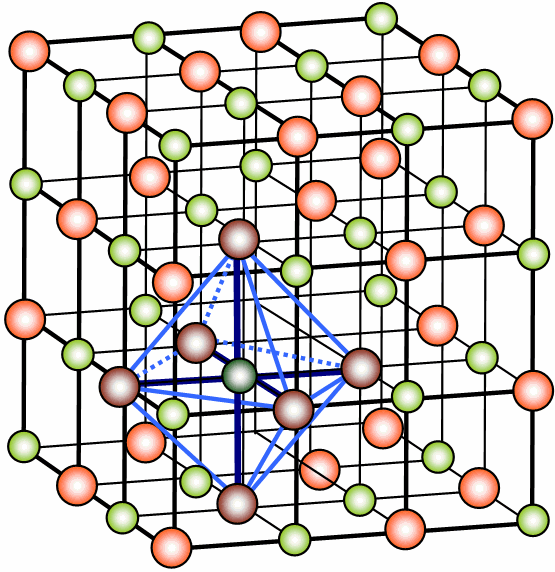
\includegraphics[width=50mm]{img/NaCl.png}
	\end{center}
	\vfill
}

\frame{
	\frametitle{}
	\begin{columns}
	\begin{column}{0.4\textwidth}
	\begin{tabular}{|l|l|}
	\hline
	\textbf{Ion} & \textbf{Vlnočet [cm$^{-1}$]} \\\hline
	\multirow{2}{*}{\ce{CO$_3^{2-}$}} & 1450-1410 \\ 
	& 880-800 \\\hline
	\multirow{2}{*}{\ce{SO$_4^{2-}$}} & 1130-1080 \\ 
	& 680-610 \\\hline
	\multirow{2}{*}{\ce{NO$_3^{-}$}} & 1410-1340 \\ 
	& 860-800 \\\hline
	\ce{PO$_4^{3-}$} & 1100-950 \\\hline
	\ce{SiO$_4^{4-}$} & 1100-900 \\\hline
	\multirow{2}{*}{\ce{NH$_4^{+}$}} & 3335-3030 \\ 
	& 1485-1390 \\\hline
	\multirow{2}{*}{\ce{MnO$_4^{-}$}} & 920-890 \\ 
	& 850-840 \\\hline
	\multirow{2}{*}{\ce{M-H}} & 2250-1700 \\
	& 800-600 \\\hline
	\ce{M-X} & 750-100 \\\hline
	\ce{M=O} & 1010-850 \\\hline
	\ce{M=N} & 1020-875 \\\hline
	\end{tabular}
	\end{column}

	\begin{column}{0.6\textwidth}
		\begin{tabular}{|l|l|}
		\hline
		\textbf{Vibrace} & \textbf{Vlnočet [cm$^{-1}$]} \\\hline
		$\nu(S=O)$ & \multirow{2}{*}{1500--1000} \\
		$\nu(S-O)$ & \\\hline
		$\nu(S-F)$ & 900--600 \\\hline
		$\delta(O-S-O)$ & 700--400 \\\hline
		$\nu(S-Cl)$ & 600--400 \\\hline
		$\nu(S-Br)$ & 400--300 \\\hline
		$\nu(P=O)$ & 1500--1200 \\\hline
		$\nu(P-O)$ & 1200--900 \\\hline
		$\nu(P-F)$ & 1000--700 \\\hline
		$\nu(P-Cl)$ & 600--400 \\\hline
		$\delta(O-P-O)$ & 650--300 \\\hline
		$\delta(F-P-F)$ & 600--350 \\\hline
		$\delta(Cl-P-Cl)$ & 300--150 \\\hline
		$\delta(Br-P-Br)$ & 200--50 \\\hline
	\end{tabular}
	\vfill
	\end{column}
	\end{columns}
}

\frame{
	\frametitle{}
	\vfill
	\begin{center}
		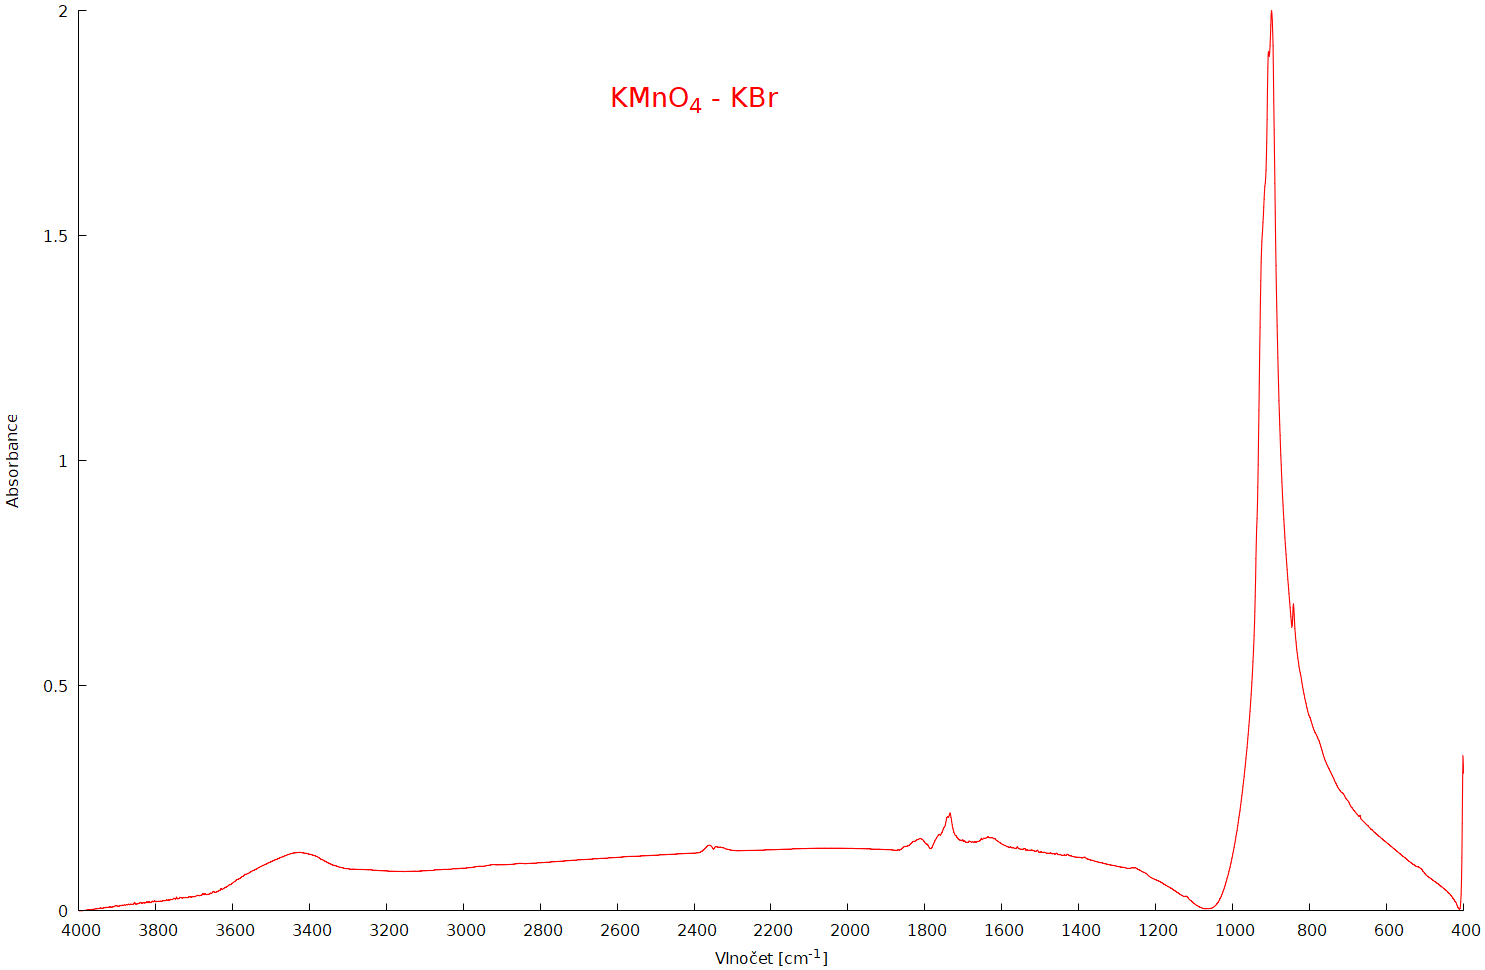
\includegraphics[width=\textwidth]{spectra/200410/KMnO4-KBr.png}
	\end{center}
	\vfill
}

\subsection{Faktory ovlivňující polohu absorpčního pásu}
\frame{
	\frametitle{}
	\vfill
	\begin{itemize}
		\item Vodíkové vazby.
		\item Izotopická substituce.
		\item Hmotnost atomů tvořících vazbu.
	\end{itemize}
	\begin{center}
	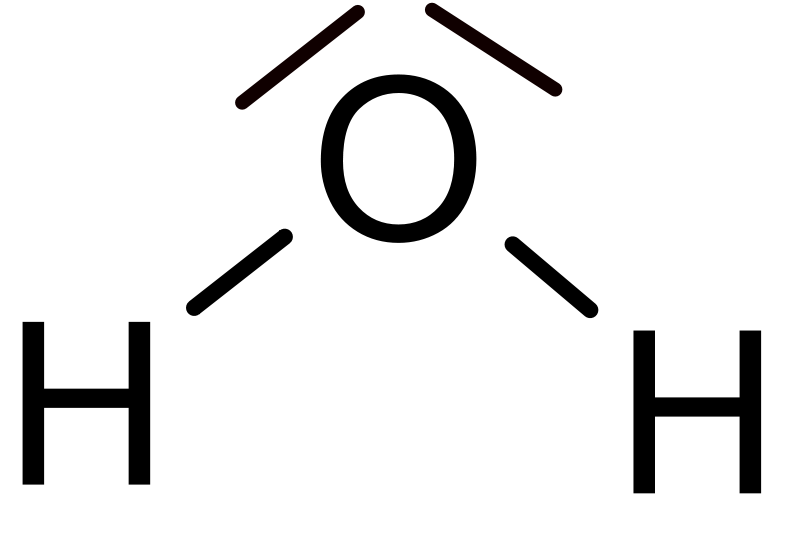
\includegraphics[height=0.2\textheight]{img/H2O.png}
	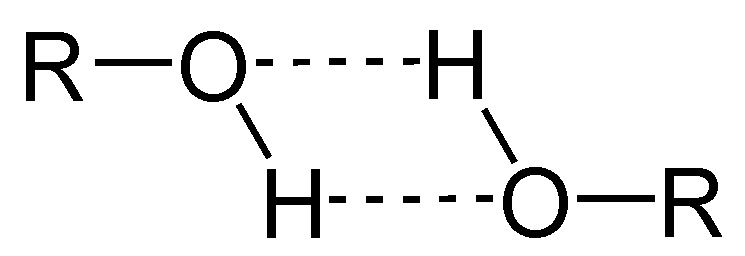
\includegraphics[height=0.2\textheight]{img/H-bonding_alcohol.png}
	\end{center}
	\vfill
}

\subsection{Vodíkové vazby}
\frame{
	\frametitle{}
	\vfill
	\begin{itemize}
		\item Přítomnost intra- i intermolekulárních vodíkových vazeb ovlivňuje sílu vazby a tím i polohu odpovídajícího pásu ve spektru.
		\item Tímto způsobem může rozpouštědlo ovlivnit vzhled spektra, např. voda, diethylether, chloroform, atd.
		\item Se vzrůstající teplotou dochází k oslabování vodíkových vazeb a tím k posunu odpovídajících pásů k vyšším hodnotám vlnočtu.
	\end{itemize}
	\begin{columns}
		\column{.8\textwidth}
		\begin{table}[H]
			\caption{Závislost vlnočtu vibrace OH skupiny fenolu na koncentraci dioxanu v \ce{CCl4}\footnotemark[1]}
			\begin{tabular}{|r@{,}l|l|l|l|}
				\hline
				\multicolumn{2}{|l|}{Konc. dioxanu [\%]} & $\nu_{OH}$ & $\nu_{OH}$ fenol-dioxan & $\Delta\nu$ \\\hline
				0 & 0 & 3611 & - & - \\\hline
				2 & 3 & 3612 & 3377 & 234 \\\hline
				22 & 1 & 3610 & 3365 & 246 \\\hline
				72 & 5 & - & 3347 & 264 \\\hline
				100 & 0 & - & 3338 & 273 \\\hline
			\end{tabular}
		\end{table}
		\column{.25\textwidth}
		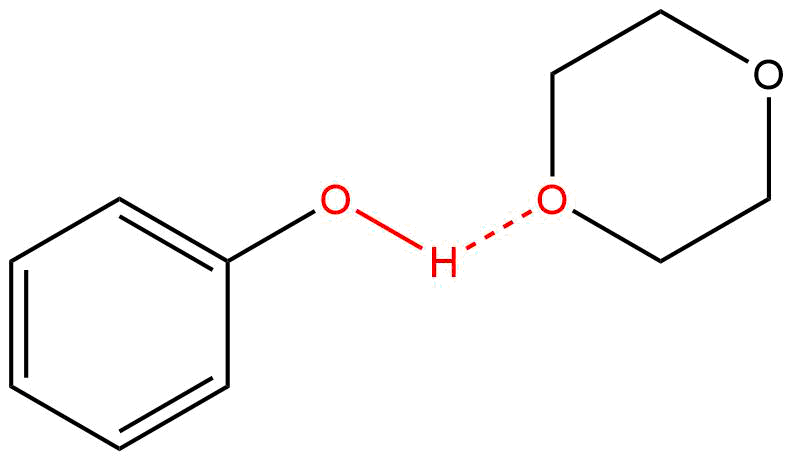
\includegraphics[width=28mm]{img/phenol-dioxane.png}
	\end{columns}
	\footnotetext[1]{\href{http://dx.doi.org/10.1021/ja00887a001}{\emph{J. Am. Chem. Soc.}, \textbf{1963}, \emph{85} (4), 371--380}}
	\vfill
	
}

\subsection{Izotopická substituce}
\frame{
	\frametitle{}
	\vfill
	\begin{columns}
		\begin{column}{0.4\textwidth}
			\begin{itemize}
				\item Izotopická substituce usnadňuje interpretaci vibračních spekter
				\item Nedochází ke změně geometrie molekuly, ale změní se hmotnost atomů a tím i poloha absorpčních pásů
				\item 	$\nu = \frac{1}{2\pi}\sqrt{k\frac{(m_1 + m_2)}{m_1m_2}}$
				\begin{itemize}
					\item k - silová konstanta vazby
					\item $m_1, m_2$ - hmotnosti atomů
				\end{itemize}
				\item Těžší izotop způsobuje posun pásu k nižším vlnočtům
			\end{itemize}
		\end{column}
		
		\begin{column}{0.5\textwidth}
			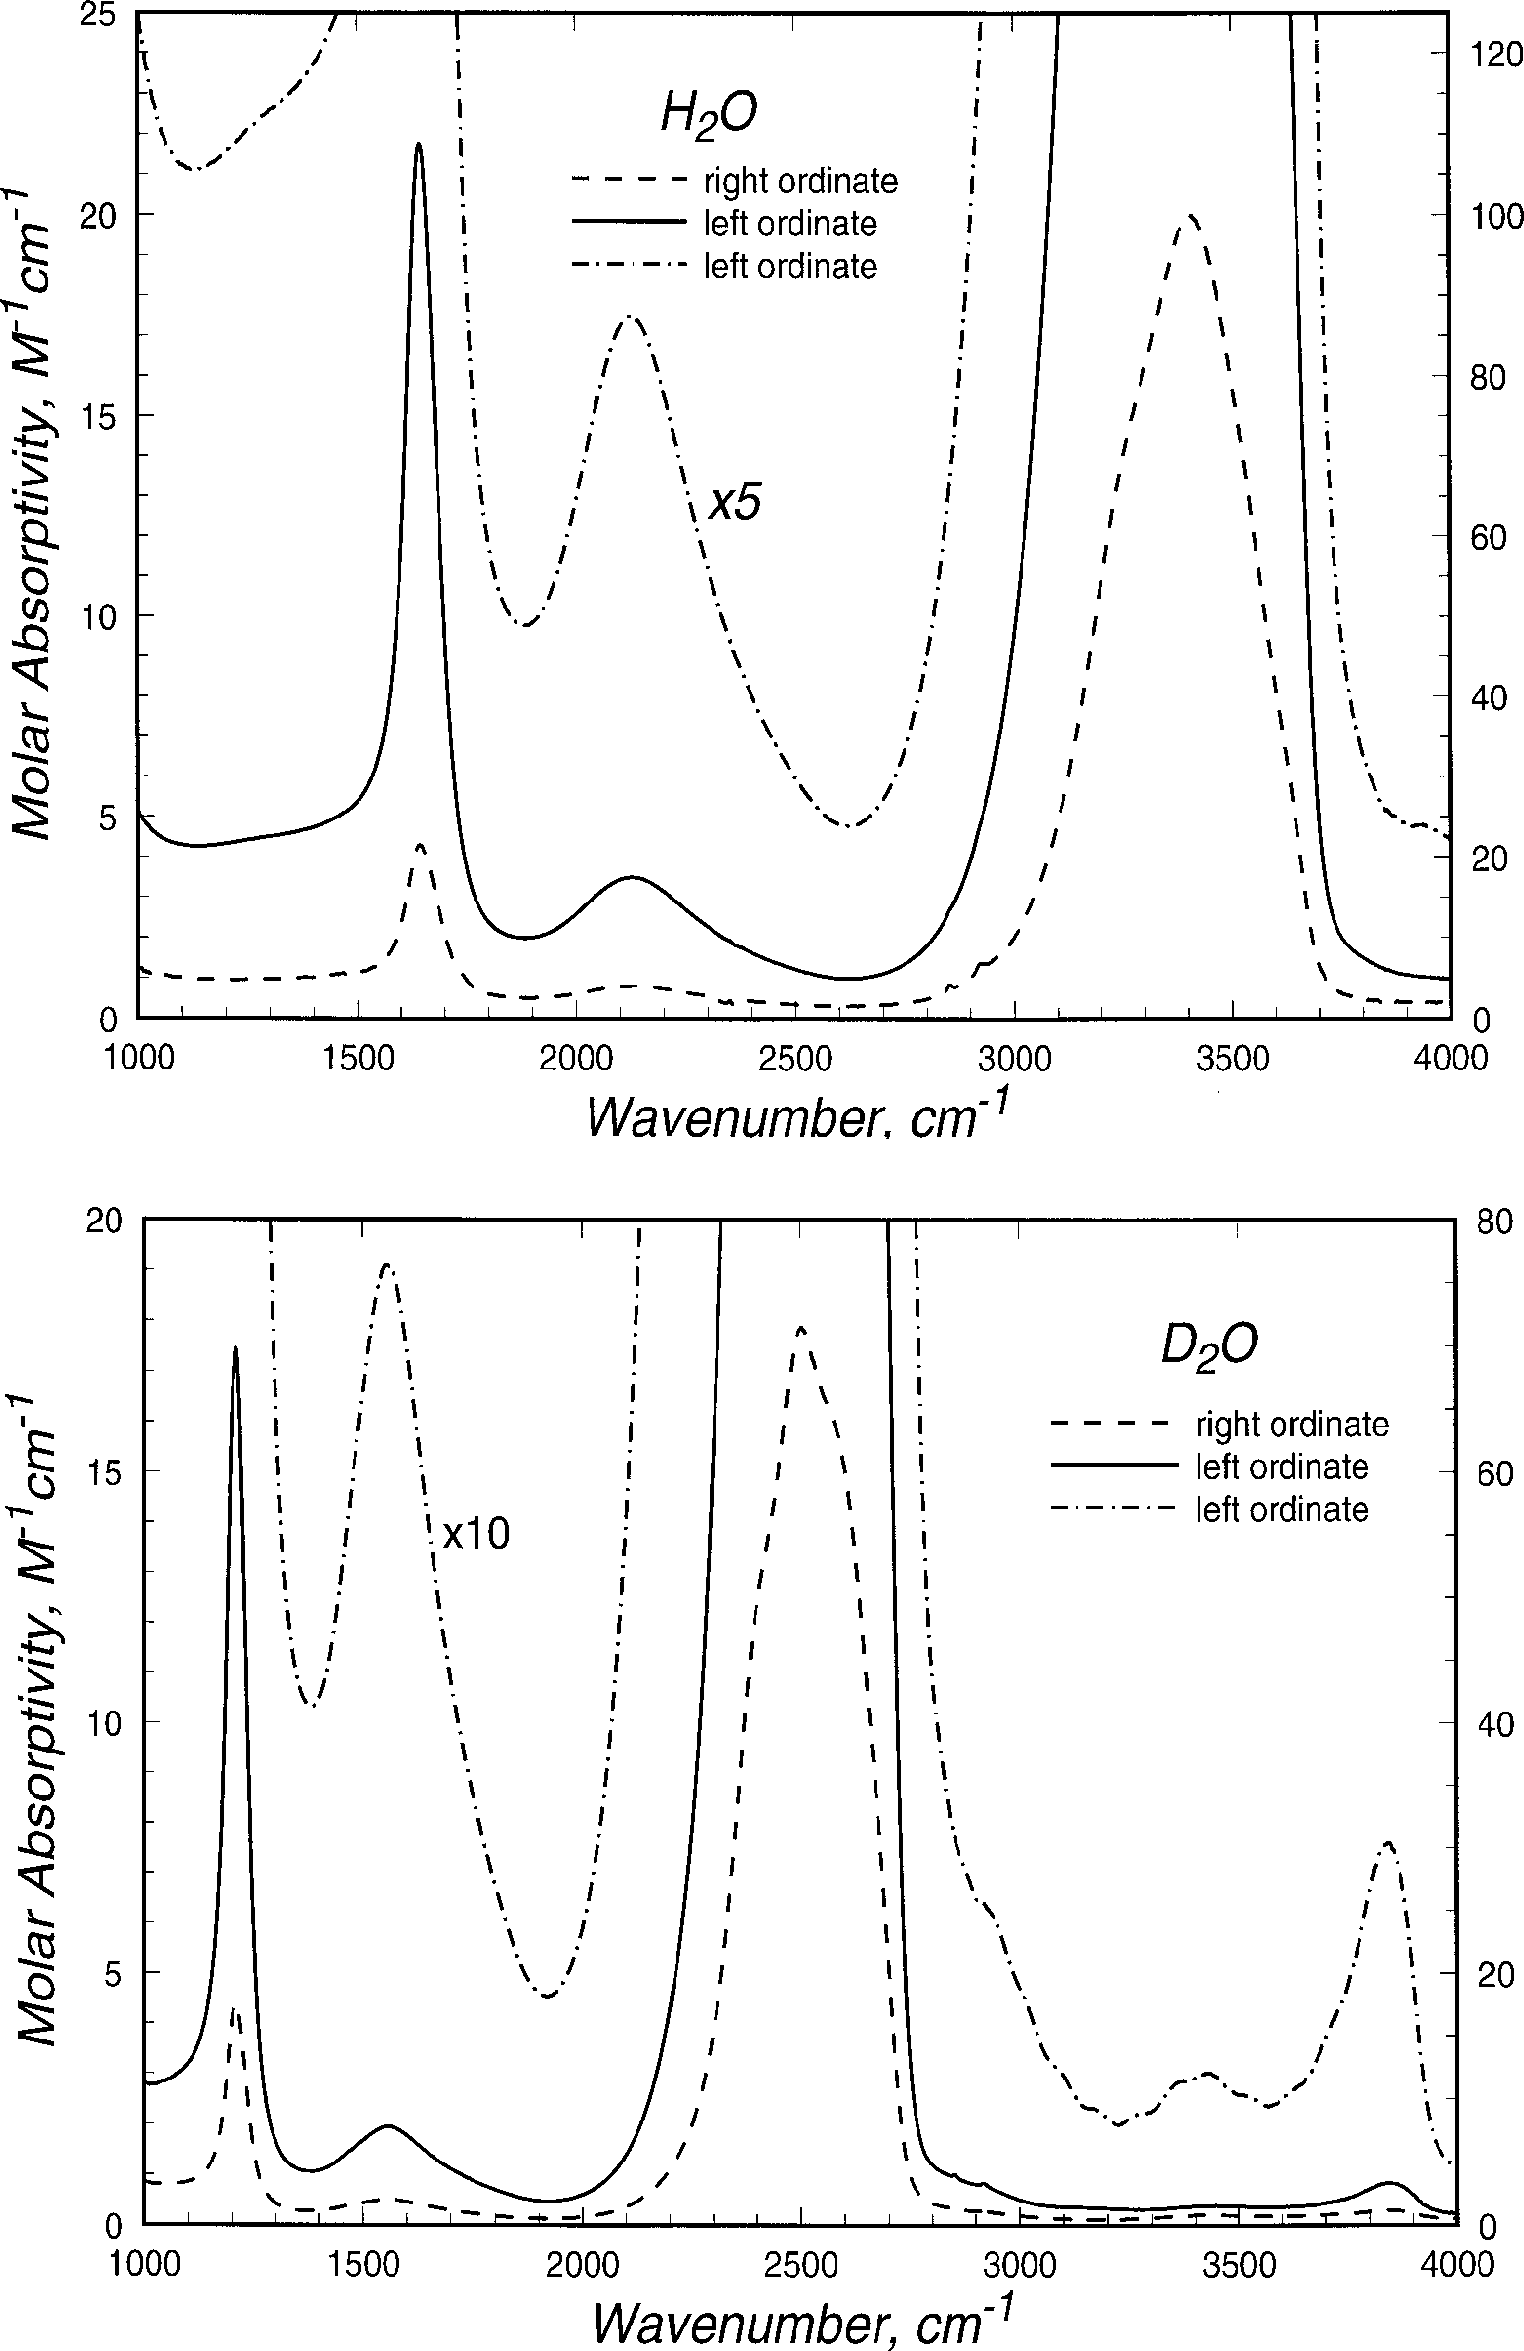
\includegraphics[width=50mm]{img/h2o-d2o.png}
		\end{column}
	\end{columns}
	\footnotetext[1]{\href{https://doi.org/10.1006/abio.1997.2136}{\emph{Anal. Biochem}, \textbf{1997}, \emph{248} (2), 234--245}}
	\vfill
}

\subsection{Halogenované sloučeniny}
\frame{
	\frametitle{}
	\vfill
	\begin{itemize}
		\item Se vzrůstající hmotností halogenu klesá hodnota vlnočtu vazby \ce{C-X}.
		\item 	$\tilde{\nu} = \frac{1}{2\pi c}\sqrt{k\frac{(m_1 + m_2)}{m_1m_2}}$
		\begin{itemize}
			\item k - silová konstanta vazby
			\item $m_1, m_2$ - hmotnosti atomů
		\end{itemize}
		\item V tabulce jsou shrnuty vibrace vazeb \ce{C-X} u alifatických uhlovodíků a vazeb \ce{B-X} v molekulách \ce{MeBX2}.
	\end{itemize}
	\begin{center}
		\begin{tabular}{|l|l||l|l|}
			\hline
			\textbf{Vazba} & \textbf{Vlnočet [cm$^{-1}$]} & \textbf{Vazba} & \textbf{Vlnočet [cm$^{-1}$]}\\\hline
			\ce{C-F} & 1150-1000 & \ce{B-F} & 1365 \\\hline
			\ce{C-Cl} & 800-700 & \ce{B-Cl} & 1018 \\\hline
			\ce{C-Br} & 700-600 & \ce{B-Br} & 965 \\\hline
			\ce{C-I} & 600-500 & & \\\hline
		\end{tabular}
	\end{center}
	\vfill
}

\subsection{NIR}
\frame{
	\frametitle{}
	\vfill
	\begin{itemize}
		\item Oblast 700-2500 nm, tj. 14~000-4~000~cm$^{-1}$.
		\item V této oblasti jsou převážně kombinační vibrace a overtony (vyšší harmonické). Ty poskytují málo intenzivní, široké  pásy, které se často překrývají.
		\item Výhodou je jednodušší instrumentace (lze využít skleněnou nebo křemennou optiku), citlivější detektory.
		\item Voda v této oblasti absorbuje relativně málo, takže ji lze použít jako rozpouštědlo.
		\item Využití v lékařství a zdravotní diagnostice, potravinářském a jiném průmyslu, astronomii, \ldots
		\item Jako měřící techniky se využívají:
		\begin{itemize}
			\item transmisní technika
			\item difuzně-reflexní technika
			\item transflexe
		\end{itemize}
	\end{itemize}
	\vfill
}

\frame{
	\frametitle{}
	\vfill
	\begin{center}
	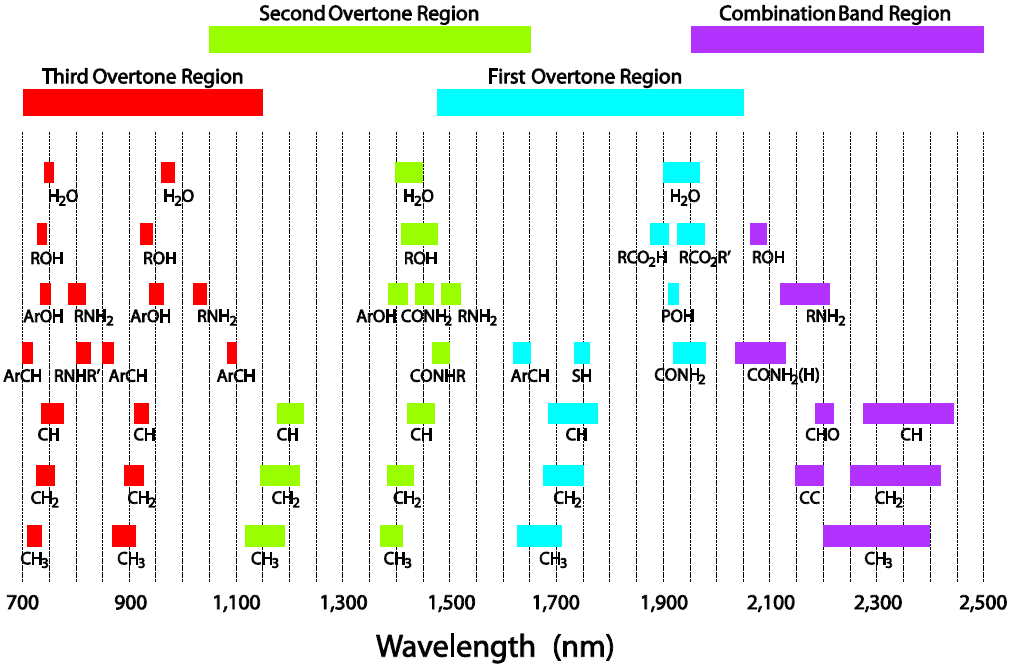
\includegraphics[width=110mm]{img/NIR-bands.png}
	\end{center}
	\vfill
}

\frame{
	\frametitle{}
	\vfill
	\begin{itemize}
	\item NIR spektrum kapalného ethanolu
	\end{itemize}
	\adjincludegraphics[width=11cm,valign=l]{img/EtOH-NIR.png}
	\vfill
}

\subsection{Ramanova spektroskopie}
\frame{
	\frametitle{}
	\vfill
	\begin{itemize}
	\item Komplementární metoda k IR spektroskopii
	\item Principem je nepružný rozptyl LASERového záření na vzorku
	\item Vhodnější pro nepolární sloučeniny
	\item Lze použít vodu jako rozpouštědlo
	\item Zpravidla užší pásy než v IR spektrech
	\item Jednoduchá příprava vzorku
	\item Měření může komplikovat fluorescence vzorku
	\item Dražší hardware
	\end{itemize}
	\vfill
}

\subsubsection{Studium struktury grafenu}
\frame{
	\frametitle{}
	\vfill
	\begin{columns}
	\begin{column}{0.55\textwidth}
	\begin{itemize}
	\item Pomocí Ramanovy spektroskopie lze studovat kvalitu grafenu a určit počet vrstev vzorku
	\item Pás D (1350~cm$^{-1}$) odpovídá poruchám ve struktuře grafenu.
	\item Pás G (1583~cm$^{-1}$) odpovídá valenčním vibracím vazeb C-C, najdeme ve všech systémech s sp$^2$ uhlíky.
	\item V případě nečistot nebo výskytu náboje na povrchu grafenu, najdeme v blízkosti pásu G i méně intenzivní pás D' (1620~cm$^{-1}$).
	\item Pás G' v oblasti 2500-2800~cm$^{-1}$ se označuje jako 2D-pás, nalezneme ho u všech systému s sp$^2$ uhlíky.
	\end{itemize}
	\end{column}
	\begin{column}{0.4\textwidth}
	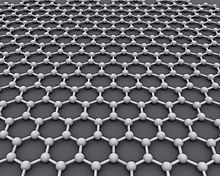
\includegraphics[width=40mm]{img/Graphen.jpg}
	\\
	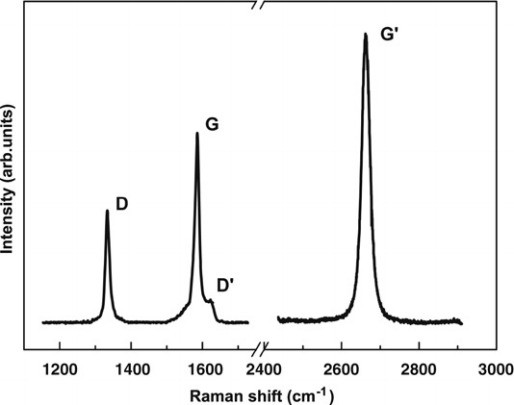
\includegraphics[width=40mm]{img/graphene-Raman.png}
	\end{column}
	\end{columns}
	\vfill
}

\section{Kvantitativní analýza}
\frame{
	\frametitle{}
	\vfill
	\begin{itemize}
		\item \emph{Lambert-Beerův zákon} -- $A_\lambda = \epsilon_\lambda l c$
		\begin{itemize}
			\item $A_\lambda$ - absorbance vzorku při vlnové délce $\lambda$
			\item $\epsilon_\lambda$ - absorpční koeficient při vlnové délce $\lambda$. Je charakteristický pro každou sloučeninu.
			\item l - délka kyvety
			\item c - molární koncentrace vzorku
		\end{itemize}
		\item Pro stanovení koncentrace se využívá \emph{kalibrační křivka}.
		\item Pás zvolený pro analýzu musí splňovat několik požadavků:
		\begin{itemize}
			\item Vysoký molární absorpční koeficient
			\item Neměl by se překrývat s jinými pásy
			\item Měl by být symetrický
			\item Závislost absorbance na koncentraci by měla být lineární
		\end{itemize}
	\end{itemize}
	\vfill
}

\subsection{Stanovení koncentrace kofeinu v roztoku}
\frame{
	\frametitle{}
	\vfill
	\adjincludegraphics[width=10cm]{img/caffeine.png}
	\adjincludegraphics[width=3cm]{img/caffeine-struct.png}
	\vfill
}

\frame{
	\frametitle{}
	\vfill
	\begin{tabular}{|l|l|}
		\hline
		\textbf{Koncentrace [mg.cm$^{-3}$]} & \textbf{Absorbance při 1656~cm$^{-1}$} \\\hline
		0 & 0.000 \\\hline
		5 & 0.105 \\\hline
		10 & 0.190 \\\hline
		15 & 0.265 \\\hline
		20 & 0.333 \\\hline
	\end{tabular}
	\adjincludegraphics[width=7cm]{img/kalibracni_krivka.png}
	\vfill
}

\section{Praktické ukázky}
\frame{
	\frametitle{}
	\vfill
	\begin{center}
		\scalebox{1.8}{\Huge Praktické ukázky}
	\end{center}
	\vfill
}

\frame{
	\frametitle{}
	\vfill
	\adjincludegraphics[width=10cm,valign=l]{spectra/mocovina-ATR.png}
	\vfill
}

\frame{
	\frametitle{}
	\vfill
	\adjincludegraphics[width=12cm,valign=l]{spectra/mocovina-SDBS.png}
	\vfill
}

\frame{
	\frametitle{}
	\vfill
	\adjincludegraphics[width=12cm,valign=l]{spectra/mocovina-nujol-SDBS.png}
	\vfill
}

\frame{
	\frametitle{}
	\vfill
	\adjincludegraphics[width=11cm,valign=l]{spectra/mocovina-scifinder.png}
	\vfill
}

\frame{
	\frametitle{}
	\vfill
	\adjincludegraphics[width=10cm,valign=l]{spectra/mocovina-ATR1.png}
	\vfill
}

\frame{
	\frametitle{}
	\vfill
	\adjincludegraphics[width=11cm,valign=l]{spectra/SO3K-ATR.png}
	\vfill
}


\frame{
	\frametitle{}
	\vfill
	\adjincludegraphics[width=11cm,valign=l]{spectra/SO3K-ATR1.png}
	\vfill
}

\frame{
	\frametitle{}
	\vfill
	\adjincludegraphics[width=11cm,valign=l]{img/Ph3SiOH-struct.png}
	\vfill
}

\frame{
	\frametitle{}
	\vfill
	\adjincludegraphics[width=11cm,valign=l]{img/Ph3SiOH-struct2.png}
	\vfill
}

\section{Literatura a odkazy}
\frame{
	\frametitle{}
	\vfill
	\begin{enumerate}
	\item STUART, Barbara. \emph{Infrared spectroscopy: fundamentals and applications.} Hoboken, NJ: J. Wiley, 2004. ISBN 9780470854280.
	\item COATES, John. Interpretation of Infrared Spectra, A Practical Approach.\emph{ Encyclopedia of Analytical Chemistry} [online]. Chichester, UK: John Wiley \& Sons, 2006 [cit. 2017-05-18]. DOI: 10.1002/9780470027318.a5606. ISBN 0470027312. Dostupné z: http://doi.wiley.com/10.1002/9780470027318.a5606
	\item \href{http://sdbs.riodb.aist.go.jp/sdbs/cgi-bin/cre\_index.cgi}{Spectral Database for Organic Compounds} -- http://sdbs.riodb.aist.go.jp/sdbs/cgi-bin/cre\_index.cgi
	\item  \href{http://webbook.nist.gov/chemistry/}{NIST Webbook Chemistry} -- http://webbook.nist.gov/chemistry/
	\end{enumerate}
	\vfill
}

\section{Závěr}
\frame{
	\vfill
	\centering \Huge
	\textbf{Děkuji za pozornost} \\[2ex]
	
	\large
	Zdeněk Moravec\\
	hugo@chemi.muni.cz \\
	\vfill
}

\end{document}